%!TEX root = ../thesis.tex
%%--------------------------------------------------------------------------
%% STATE OF THE ARTS
%%--------------------------------------------------------------------------



% --------------------------------------------------------------------------- %
% ---------------------------------- INTRO ---------------------------------- %
% --------------------------------------------------------------------------- %


\section{Introduction}
\label{sec:sota_intro}
As described in the Introduction (\ref{chap:intro}) our thesis has two different topics. The first is the development of a system to create cloud infrastructure experimentation environments for developers and researchers. The second is the implementation of an OpenStack module to allow one to test consolidation algorithms to improve the resource allocation efficiency of the cloud infrastructure and, as a result, its energy efficiency.\\
For that reason this chapter is divided into two sections in which we are going to present the state of the arts of Cloud Test Environments and of Virtual Machines Consolidation.


% ------------------------------------------------------------------------- %
% --------------------------- VMs consolidation --------------------------- %
% ------------------------------------------------------------------------- %

\section{Virtual Machine consolidation}
\label{sec:sota_vm_cons}
At its most basic essence, cloud computing can be seen as a means to provide developers with computation, storage, and networking resources on-demand, using virtualization techniques and the service abstraction \cite{Armbrust:2010ee}. The service abstraction makes the cloud suitable for use in a wide variety of scenarios, allowing software developers to create unique applications with very small upfront investments, both in terms of capital outlays and in terms of required technical expertise. Thanks to Cloud Computing, Internet software services have rightfully taken their place as important enablers in areas of great social importance, such as ambient assisted living \cite{Zhang:2011dq}, education \cite{Sultan:2010fd}, social networking \cite{Chard:2010eh}, and mobile applications \cite{Fernando:2013ip}.\\
Managing a Cloud Infrastructure, however, presents many unique challenges. For example, there has been a lot of focus in the last few years on Virtual Machines Placement and Server Consolidation, given the role they play in optimizing resource utilization and energy consumption \cite{Feller:2012kf}, \cite{Goudarzi:2012gw}. Virtual Machine (VM) Placement \cite{Meng:2010im}, \cite{Xu:2010df} defines how a cloud installation decides on which physical server to create a new virtual machine, when one is requested. Server Consolidation techniques \cite{Wuhib:2012vq}, \cite{Corradi:2014fe}, on the other hand, allow a cloud provider to perform periodical run-time optimizations, for example through the live migration of VMs. The goal is always to desist from having too many under-utilized hardware resources given a specific workload, and to achieve this without compromising the quality of service that is offered to the cloud’s customers.\\
Dynamic consolidation of Virtual machines is enabled by \textit{live migration}, that is the capability to move a running Virtual Machine from one physical hosts to another with no downtime and no disruptions for the user. Thanks to dynamic Virtual Machine consolidation it is possible to minimize the number of active hosts, and to remove Virtual Machines from hosts when they become overloaded therefore avoiding performance degradation.

With regard to Virtual Machine Consolidation a lot of solutions, algorithms and techniques have been proposed in literature \cite{He:2012jr}, \cite{Wuhib:2012vq}, \cite{Corradi:2014fe}; we decided to focus on four interesting papers described in sections \ref{sec:sota_ga}, \ref{sec:sota_holistic}, \ref{sec:sota_game_theroy} and \ref{sec:sota_mutli_agent}. The section \ref{sec:sota_neat} is dedicated to the only attempt within the state of the art to apply Virtual Machine consolidation in the OpenStack world.

\subsection{Genetic Algorithm}
\label{sec:sota_ga}
In the paper \textit{Toward Virtual Machine Packing Optimization Based on Genetic Algorithm}\cite{Nakada:2009in} the authors explain how they modeled the problem of Virtual Machines consolidation as a bin packing problem and how they structured a Genetic Algorithm to deal with it. A Genetic Algorithm is a heuristic algorithm, i.e., a type of technique that is often used to address NP-hard problems such as the bin packing problem. A GA is a kind of machine learning that takes inspiration from the concept of evolution observed in biological environments, from which it borrows a lot of terms such as Chromosome, Mutation or Population.\\
The paper in question defines the concepts of a Genetic Algorithm for the Virtual Machine packing problem as follows:
\begin{description}
  \item[Chromosome] It represents a physical node, and in particular the list of hosted virtual machines.
  \item[Crossover] They use a One-Point Crossover that randomly cuts two chromosomes and mix them. They also implement a repair function to fix the inconsistent children thus obtained.
  \item[Mutation] They randomly exchange two positions between them.
  \item[Initial Population Generation] They generate the initial population using a Minimal Generation Gap method.
  \item[Objective Function] The unspecified objective function is said to be designed with parameters and weights in mind, such as SLA (Service level agreement) violations, number of active nodes, and number of migrations applied.
\end{description}

The experimentation environment and the simulation tests are not described in a detailed way and there are no data results to prove the soundness of the approach. Still, the idea of implementing a Genetic Algorithm to solve the consolidation problem is interesting, and possibly very efficient and useful; for these reasons we decided to take inspiration from it and implement a Genetic Algorithm, to be applied in an OpenStack test environment deployed with aDock, as described in section \ref{sub:algs_ga}.

\subsection{Holistic Approach}
\label{sec:sota_holistic}
The paper \textit{Energy Management in IaaS Clouds: A Holistic Approach} published during the IEEE Fifth International Conference on Cloud Computing in 2012 presents energy management algorithms and a holistic energy-aware Virtual Machine management framework for private clouds called Snooze.\\
The system architecture described by the authors (see figure \ref{fig:snooze_arch} on page \pageref{fig:snooze_arch}) is divided in three layers:
\begin{description}
  \item[Physical layer] It contains clusters of nodes; each is controlled by a Local Controller (LCs).
    \begin{itemize}
      \item \textit{Local Controller} - They enforce Virtual Machines and host management commands coming from the GM (Group Manager, see below). Moreover, they monitor VMs, detect overload/underload anomalous situations and report them to the assigned GM.
    \end{itemize}
  \item[Hierarchical layer] It allows to scale the system and is composed of fault-tolerant components: Group Managers (GMs) and a Group Leader (GL).
      \begin{itemize}
      \item \textit{Group Leader} - One GL oversees the GMs, keeps aggregated GM resource summary information, assigns LCs to GMs, and dispatches VM submission requests to the GM.
      \item \textit{Group Managers} - Each of them manages a subset of physical hosts; they retrieve resource information and send commands, received by the GL, to the LCs.
      \end{itemize}
  \item[Client layer] It provides the user interface and it is implemented by a predefined number of replicated Entry Points (EPs).
\end{description}

The system addresses the scheduling problem both at the GL level, where VM to GM dispatching is done based on the GM resource summary information in a round-robin way, and at the GM level where the real scheduling decisions are made. In addition to the \textit{placement policies}, which are applied when a new VM is requested, the work also supports \textit{relocation policies}, which are called when overload or underload events arrive from LCs, and \textit{consolidation policies}, which are called periodically according to one interval that is specified by the system administrator.\\
The paper proposes an algorithm for both overload and underload relocation policy. They both take as input the overloaded/underloaded LC along with its associated VMs and a list of LCs managed by the GM and output a Migration Plan (MP) which specifies the new VM locations.\\
The algorithm proposed for the consolidation follows an all-or-nothing approach and attempts to move VMs from the least loaded LC to a non-empty LC with enough spare capacity.  LCs are first sorted in decreasing order based on their estimated utilization. Afterwards, VMs from the least loaded LC are sorted in decreasing order, placed on the LCs starting from the most loaded one and added to the migration plan. If all VMs could be placed the algorithm increments the number of released nodes and continues with the next LC. Otherwise, all placed VMs are removed from the LC and MP and the procedure is repeated with the next loaded LC. The algorithm terminates when it has reached the most loaded LC and outputs the MP, number of used nodes, and number of released nodes\cite[p.~208]{Feller:2012kf}.\\
In section \ref{sub:algs_holistic} we describe how we implemented this algorithm in our system and the result obtained with our configuration.


\begin{figure}[!ht]
\centering{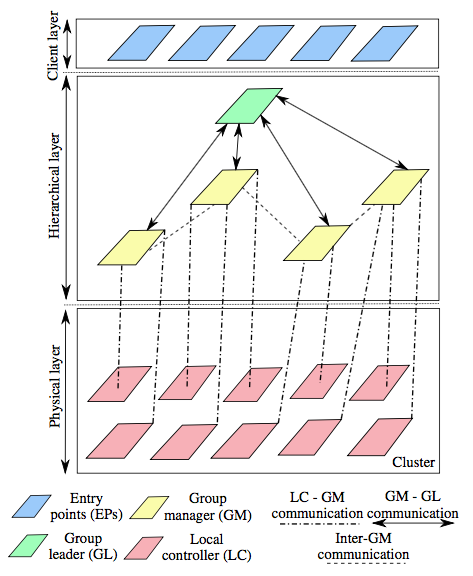
\includegraphics[width=\textwidth]{images/snooze_arch.png}}
\label{fig:snooze_arch}
\caption{The Snooze architecture \cite{Feller:2012kf}}
\end{figure}

\subsection{Game Theory Approach}
\label{sec:sota_game_theroy}
The paper \textit{A Game Theory Approach to Fair and Efficient Resource Allocation in Cloud Computing} proposes a game theoretic resources allocation algorithm that considers the fairness among users and the resources utilization for both \cite{Xu:2014do}.\\
The four main components of the proposed cloud resource management system are:
\begin{description}
  \item[CEM - Cloud Environment Monitor] This component retrieves information like host names and IP addresses about physical servers, and monitors their statuses (starting, running, shutdown) and the consumption of CPU, memory, and disk storage.
  \item[RC - Register Center] Every physical server in cloud data center should register its information to RC for connection and management.
  \item[IM - Infrastructure Manager] It is responsible for deploying and managing the virtualized infrastructures, such as creating and releasing virtual machines.
  \item[CC - Control Center] It is the control center to provide the most appropriate decision about resource allocating.
\end{description}

CEM monitors the statuses and resource consumptions for physical servers registered in RC. Once a new physical server joins the cloud, information like its MAC address and its IP address will be registered to RC. When a user sends a service request to the cloud, the resource requirements this request will be received by CC. CC makes an intelligent resource allocation decision based on the information collected by CEM. The allocation decision is executed by IM to manage the physical servers and place the virtual machines.\cite[p.~3]{Xu:2014do}

They experimented a FUGA (Fairness-Utilization tradeoff Game Algorithm) on a server cluster composed of 8 nodes and compared it to the Hadoop\footnote{A framework that allows for the distributed processing of large data sets across clusters of computers using simple programming models. \url{http://hadoop.apache.org}} \textit{fair scheduler}\footnote{``Fair scheduling is a method of assigning resources to jobs such that all jobs get, on average, an equal share of resources over time.'', \url{hadoop.apache.org/docs/r1.2.1/fair_scheduler.html}}. They showed that it is possible to achieve an optimal tradeoff between fairness and efficiency compared with the evaluation of the Hadoop scheduler.

\subsection{Multi-agent Virtual Machine Management}
\label{sec:sota_mutli_agent}
The solution presented in the paper \textit{Multi-agent Virtual Machine Management Using the Lightweight Coordination Calculus} specifies the migration behavior of Virtual Machines within, and between cloud environments. It uses a Lightweight Coordination Calculus to provide an executable, declarative specification of an agent interaction model\cite{Anderson:2013bh}.

The proposed system is distributed between nodes; it doesn't have a central controller that could represent a single point of failure or a bottleneck. Agents located on the physical machines negotiate VM transfer between themselves, without referencing any centralized authority\cite[p.~124]{Anderson:2013bh}.

The framework designed by the authors provides different types of interaction models by which it is possible to implement a wide range of algorithms and policies to support different situations.

\subsection{Neat}
\label{sec:sota_neat}
OpenStack, at the state of the art, provides a comprehensive and efficient Virtual Machines Placement system. As described in section \ref{par:openstack_nova_sched}, it is part of the \code{nova-scheduler} module. However, with regard to Virtual Machines Consolidation, OpenStack does not include any official solution or plans to include it.\\
The only project that tried to bring Virtual Machine consolidation concepts to OpenStack is Neat\footnote{\url{github.com/beloglazov/openstack-neat}}. It is defined as a framework for dynamic and energy-efficient consolidation of virtual machines in OpenStack clouds \cite{beloglazov2014openstack}.\\
OpenStack Neat approaches the consolidation problem by splitting it in four sub-problems~\cite[p.~3]{beloglazov2014openstack}:
\begin{itemize}
  \item  Deciding whether a host is \textit{underloaded}. In this case all Virtual Machines should be migrated from it, and the host should be switched to a low-power mode. 
  \item Deciding whether a host is \textit{overloaded}. In this case some Virtual Machines should be migrated from it to an other active host or a host should be reactivated to avoid violating the QoS requirements.
  \item Selecting the Virtual Machines to migrate from an overloaded host.
  \item Placing the selected Virtual Machines on an other active host, or on a reactivated one.
\end{itemize}

\begin{figure}[!ht]
\centering{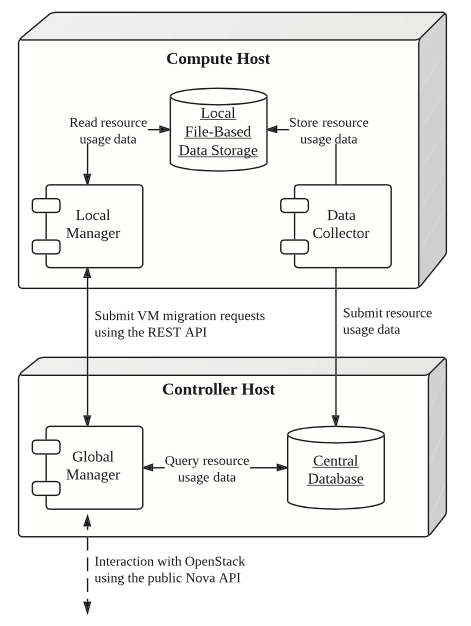
\includegraphics[width=\textwidth]{images/neat_arch.png}}
\label{fig:neat_arch}
\caption{The OpenStack Neat architecture \cite{beloglazov2014openstack}}
\end{figure}

Figure \ref{fig:neat_arch}~\cite[p.~7]{beloglazov2014openstack} represents the architecture of OpenStack Neat: it is mainly composed by a \textit{Global Manager} installed on the Controller node, and by a \textit{Local Manager} and a \textit{Data Collector} installed on every Compute node. The \textit{Global Manager} is responsible for making global management decisions such as mapping Virtual Machine instances to hosts, and initiating Virtual Machines live migrations; the \textit{Local Manager} makes local decisions such as deciding that the host is underloaded or overloaded and selecting Virtual Machines to migrate to other hosts; lastly the \textit{Data Collector} is responsible for collecting Virtual Machines and hypervisors resource usage data and for then storing the data locally and submitting it to the central database, which can also be distributed.\\
One of the main characteristics of OpenStack Neat is that it is designed to be distributed and external to OpenStack, in fact it acts independently of the base OpenStack platform and applies Virtual Machines consolidation by invoking OpenStack's public APIs. For that reason it has to be installed separately from OpenStack, following the limited instructions present on the GitHub page of the project\footnote{\url{github.com/beloglazov/openstack-neat}} and can not take advantage of tools like DevStack (see \ref{chap:openstack_devstack} on page \pageref{chap:openstack_devstack}) that automates the deploy and configuration of an OpenStack installation. \\


% -------------------------------------------------------------------------- %
% ------------------------- CLOUD TEST ENVIRONMENT ------------------------- %
% -------------------------------------------------------------------------- %

\section{Cloud test environments}
\label{sec:sota_test_env}

When provisioning a cloud we need to be able to test different environment configurations and algorithms, to analyze the behavior of new code that need to integrate with the environment, and to benchmark and collect data for research and experimentations. Unfortunately it can be expensive and complex to create and manage a cloud test environment in terms of time, resources and expertises, especially if the hardware resources like server machines or network infrastructures are limited. Fully understanding and handling an OpenStack installation is not easy, especially for non sysadmins like developers or researchers; it has a high learning curve and often a lot of time is needed to achieve the desired results.\\
There are some tools that reduce the impact of these complications are and make the process of setting up a cloud infrastructure experimentation environment easier and more manageable.
The growing need of advanced system management have made configuration management tools, such as Chef and Puppet, have become increasingly mainstream. These tools provide domain-specific declarative languages for writing complex system configurations, allowing developers to specify concepts such as ``what software packages need to be installed'', ``what services should be running on each hardware node'', etc. More recently OpenStack has started collaborating both with Chef (see section \ref{sub:sota_chef}) and Puppet (see section \ref{sub:sota_puppet}) to create new means to configure and deploy fully-functional OpenStack environments on bare-metal hardware, as well as on Vagrant virtual machines. The combination of a system management tool, like Chef or Puppet, and Vagrant can be used to setup a virtualized experimentation environment. However, these are complex sysadmin tools that require strong technical skills.\\
Below we present them and highlight their main features, as well as their strengths and weaknesses with respect to the topic of our thesis.

\subsection{Vagrant}
\label{sub:sota_vagrant}
Vagrant\footnote{\url{www.vagrantup.com}} is a virtualization framework for creating, configuring and managing development environments, written in Ruby. It is a wrapper around virtualization software such as VirtualBox, KVM, VMware and could be used together with configuration management tools such as Chef and Puppet.
Thanks to an online repository \footnote{\url{www.vagrantcloud.com}} it is possible to automatically download a Vagrant Box and run it with a single command: \code{vagrant up vagrant-box-name}.
It is also possible to create and configure custom Vagrant Box by simply writing a \code{Vagrantfile}:
\begin{lstlisting}[
  float,
  floatplacement=H,
  language=Ruby,
  numbers=none,
  caption={\texttt{Vagrantfile} example},
  label={lst:vagrantfile_example},
  ]
box      = 'trusty64'
url      = 'http://files.vagrantup.com/precise32.box'
hostname = 'customtrustybox'
domain   = 'example.com'
ip       = '192.168.0.42'
ram      = '2048'

Vagrant::Config.run do |config|
  config.vm.box = box
  config.vm.box_url = url
  config.vm.host_name = hostname + '.' + domain
  config.vm.network :hostonly, ip

  config.vm.customize [
    'modifyvm', :id,
    '--name', hostname,
    '--memory', ram
  ]
end
\end{lstlisting}
Provisioners in Vagrant allows one to automatically install and configure software in a Vagrant Box as part of the \code{vagrant up} process. Therefore it is easier to start with a base Vagrant Box, adapt it to your needs and eventually share it with other developers who can reproduce the same virtual development environment.\\
Vagrant is used together with configuration management software such as Chef and Puppet to create repeatable and easy to setup development and test environments that rely on Virtual Machines.


% ---------------------------------- CHEF ---------------------------------- %

\subsection{Chef}
\label{sub:sota_chef}

\subparagraph{Description}
\label{subp:sota_chef_desc}

Chef\footnote{\url{www.chef.io}} is a configuration management tool used to streamline the task of configuring and maintaining servers in a cloud environment. It can be integrated with cloud-based platforms such as Rackspace, Amazon EC2, Google Cloud Platform, OpenStack and others. It is written in Ruby and Erlang and uses a domain-specific language (DSL)\footnote{A programming language specialized to a particular application domain.} for writing configuration files called \textit{recipes}. \textit{Recipes} are used to define the state of certain resources\footnote{A resource state is a combination of installed software, running services, and configurations.}, and everything that is required to configure the different parts of the system. They state what software should be installed (together with any required dependencies), services that should be run or files that should be written. Given a \textit{recipe} Chef ensures that all the software is installed in the right order and that each resource state is reached, eventually correcting those resources in a undesired state; \textit{recipes} can be collected into \textit{cookbooks} to be more maintainable and powerful. In addition Chef offers a centralized hub, called Chef Supermarket\footnote{\url{supermarket.chef.io}}; it collects a large number of \textit{cookbooks} from the community that are freely downloadable.\\
A base installation of Chef comprises three main components: a \code{chef-server} that orchestrates all the Chef processes, multiple \code{chef-clients} found on all the servers, and the user workstation that communicates with the Chef Server to launch commands.\\
To simplify communication with the \code{chef-server} Chef provides a command-line tool called Knife that helps users manage nodes, \textit{cookbooks} and \textit{recipes}.

\subparagraph{Chef and OpenStack}
\label{subp:sota_chef_openstack}

Chef and OpenStack can be combined and used together in different ways, many of which have a different goal compared to our thesis. It is possible, in fact, to deploy and manage a production OpenStack installation running on multiple servers and supervised by a Chef Server (using the subcommand \code{knife openstack}) to control the OpenStack APIs through Chef and to instantiate new physical servers with a \code{chef-client} or turn some off (\code{knife openstack server create / delete}).
In this situation you can achieve a ``1 + N'' OpenStack configuration. In this case the OpenStack services are predefined and you cannot configure an ad hoc configuration.
It is also possible to have an ``All-in-One'' configuration, where all the OpenStack services are installed on a single node.\\
These configurations can be achieved with the help of Vagrant that will cover all the steps to install OpenStack on a virtual machine and configure all its services (excluded Block Storage, Object Storage, Metering, and Orchestration). Within the OpenStack chef-repo\footnote{\url{https://github.com/stackforge/openstack-chef-repo}} there is a \textit{recipe} to configure a VirtualBox virtual machine that will host and All-in-One installation. Here is a part of it:

\begin{lstlisting}[
  float,
  floatplacement=H,
  language=Ruby,
  numbers=none,
  caption={Recipe to run an ``All-in-One'' configuration (\texttt{aio-nova.rb})},
  label={lst:aio_recipe},
  ]
machine 'controller' do
  add_machine_options vagrant_config: controller_config
  role 'allinone-compute'
  role 'os-image-upload'

  chef_environment 'vagrant-aio-nova'
  file('/etc/chef/openstack_data_bag_secret',
       "#{File.dirname(__FILE__)}/.chef/encrypted_data_bag_secret")
  converge true
\end{lstlisting}

Of course it is possible to setup a ``1 + N'' configuration using different \code{Vagrantfiles} to create and configure one VM for the Controller and N VMs for the Compute nodes. However it is unlikely to succeed in running a lot of VMs on the same host, especially if they contain a fully functional OpenStack installation, since a Virtual Machine typically requires a significant amount of resources to operate.

\subparagraph{Pros and Cons}
\label{subp:sota_chef_pro_cons}

Chef is a very powerful tool to create, manage and configure cloud environments, and it offers a lot of functionalities to structure the desired architecture. In combination with Vagrant can also be used to setup test environments for development or research purposes.\\
However, with regard to this last aspect, it has several limitations:
\begin{itemize}
\item \textit{Performance}: because VMs are very resource greedy it is very difficult to achieve a ``1 + N'' configuration for development or research purpose on a single machine. On the other hand the ``All-in-One Compute'' solution that allows a full OpenStack installation on a single Virtual Machine is very simplistic and doesn't represent a real environment setting.
\item \textit{Lack of customization}: at the state of the art all of the described solutions install both the Controller node and the Compute node with a predefined set of installed services (in practice all the OpenStack service excluded Object Storage, Metering, and Orchestration are installed) so it is not possible to setup the environment with more or less services or new ones. In our case, in fact, we need to be able to decide which OpenStack services to install (for example we don't install OpenStack Network as a Service module, \code{Neutron}), as well as to implement a new one and install it (see chapter \ref{chap:consolidator} regarding our Consolidator service).
\end{itemize}


% ---------------------------------- PUPPET ---------------------------------- %


\subsection{Puppet}
\label{sub:sota_puppet}

\subparagraph{Description}
\label{subp:sota_puppet_desc}

Similarly to Chef (described in section~\ref{sub:sota_chef}) Puppet\footnote{\url{www.puppetlabs.com}} is a configuration management system that allows you to define the state of a cloud infrastructure, which it will then automatically enforce.\\
Puppet uses a declarative model where one defines the resource states; its manifest files are written in a Ruby-like DSL. Configuration files are enclosed in \textit{modules}, self-contained bundles of code and data that are easy to share and reuse. There are a large amount of them on the Puppet Forge\footnote{\url{forge.puppetlabs.com}} repository.\\
Puppet is structured in a master-slave architecture: the master serves the manifests and the files, and the clients polls the master at specific intervals of time to get their configurations so that the master never pushes nothing to them.


\subparagraph{Puppet and OpenStack}
\label{subp:sota_puppet_openstack}

As seen for Chef, Puppet can be very useful when dealing with OpenStack installation and maintenance. To configure and deploy an OpenStack infrastructure with the help of Puppet one can download appropriate \textit{modules} from Puppet Forge; this simplifies most of the operations such as OpenStack instances provisioning, configuration management and others.
The module is \code{puppetlabs-openstack}\footnote{\url{github.com/puppetlabs/puppetlabs-openstack}}; using this module it is possible to deploy both a multi-node and an all-in-one installation. Compared to Chef, Puppet is a bit more flexible because it allows you to control more details about the OpenStack services that are to be installed on every node; for example, you can use the following instructions in the Puppet's manifest file of a node to achieve different results. In listing \ref{lst:manifest_controller} we show a portion of a manifest file for a controller node, while in listing \ref{lst:manifest_compute} we show it for a compute node.

\begin{lstlisting}[
  float,
  floatplacement=H,
  language=Ruby,
  numbers=none,
  caption={Portion of a manifest file for a controller node},
  label={lst:manifest_controller},
  ]
node 'control.localdomain' {
  include ::openstack::role::controller
}
\end{lstlisting}

\begin{lstlisting}[
  float,
  floatplacement=H,
  language=Ruby,
  numbers=none,
  caption={Portion of a manifest file for a compute node},
  label={lst:manifest_compute},
  ]
node 'storage.localdomain' {
  include ::openstack::role::storage
}

node 'network.localdomain' {
  include ::openstack::role::network
}

node /compute[0-9]+.localdomain/ {
  include ::openstack::role::compute
}
\end{lstlisting}

Obviously, it is possible to configure multiple nodes to run in multiple Virtual Machines that are configured and launched with Vagrant and deploy the various OpenStack components with \code{puppetlabs-openstack}. This solution, is clearly difficult to achieve on a machine with a limited amount of resources; however also on a more powerful server machine this solution it is slightly feasible and scalable.

\subparagraph{Pros and Cons}
\label{subp:sota_puppet_pro_cons}
Puppet is an extremely powerful and mature tools for automated cloud infrastructure deploying: it streamlines the entire process and automates every step of the software delivery process.\\
However from our point of view we are more interested in knowing how it behaves when a single developer or a researcher needs to deploy a cloud infrastructure on a single machine with limited amounts of resources (a development workstation for example) and he/she has little sysadmin skills. With regard to this aspect Puppet used with Vagrant has some key limitations:

\begin{itemize}
\item \textit{Performance}: A single Virtual Machine generally need a remarkable amount of resources, especially to host an OpenStack installation; for this reason it is very unlikely that one will be able to run on a single machine the number of Virtual Machines needed to deploy a realistic multi-node installation of OpenStack. Once again ``all-in-one'' solution is not sufficiently realistic, especially when testing algorithms or portions of code that involve multiple nodes.
\end{itemize}

% ---------------------------------- CHEF ---------------------------------- %

\subsection{Docker}
\label{sub:sota_docker}
Docker\footnote{\url{www.docker.com}} is an open platform for developers and sysadmins to build, ship, and run distributed applications. Its core is the Docker Engine: it exploits Linux containers to virtualize a guest Operating System on a host avoiding the considerable amount of resources necessary to run Virtual Machines.\\
The main difference between the Docker solution and Virtual Machines solution lie in the way in which the hypervisor and the Docker Engine manage the guest Operating System. A Virtual Machine, as shown in figure ~\ref{fig:docker_vm} on page~\pageref{fig:docker_vm}, hosts a complete Operating System including application, dependency libraries, and, more important, the kernel; the Docker Engine, on the other hand, runs as an isolated process in userspace on the host operating system and allows all the guest containers to share the kernel. Thus, it enjoys the resource isolation and allocation benefits of Virtual Machines, but is much more portable and efficient; for our goals this aspect allows us to run at the same time a larger number of containers compared to what we are able to achieve with Virtual Machines and also to ship pre-built images of our modules.\\
To configure and build a container image you have to write a Dockerfile, that is a text document containing all the commands which you would have normally executed manually in order to take the container to the desired state, and then call \code{\$ sudo docker build .} from the directory containing the file. The command \code{\$ sudo docker run} will finally launch the container.\\
Docker offers an online platform called Docker Hub\footnote{\url{hub.docker.com}} where you can upload both Dockerfile and pre-built container images to streamline the sharing process.
    
\begin{figure}[!ht]
\centering{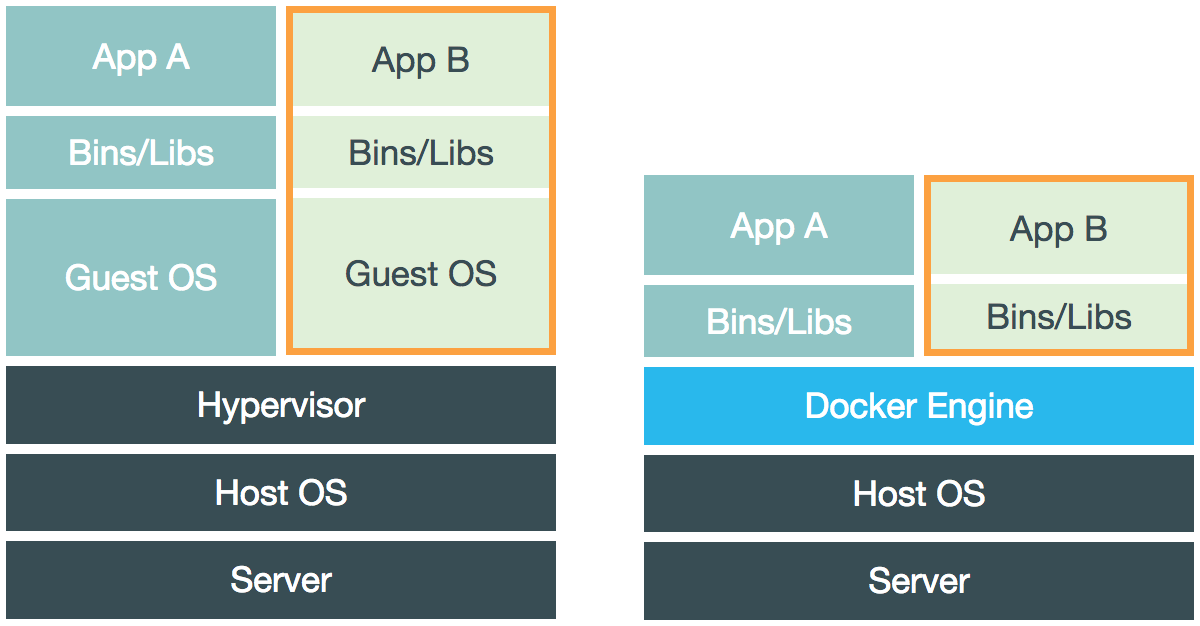
\includegraphics[width=\textwidth]{images/docker_vs_vm.png}}
\label{fig:docker_vm}
\caption{Hypervisor and Docker Engine}
\end{figure}

% ------------------------------- DOCKENSTACK ------------------------------- %

\subsection{Dockenstack}
\label{sub:sota_dockenstack}
One of the first attempts to create a cloud test environment based on OpenStack and Docker is Dockenstack\footnote{\url{github.com/ewindisch/dockenstack}}. It is an independent and not actively supported project, but is a good starting point to show the potential derived from using Docker.\\
The project is basically composed of a Dockerfile and a bunch of scripts that will setup and configure an OpenStack installation using DevStack in a Docker container.\\
A pre-built image is available on Docker Hub, so with the command \code{docker run -privileged -t -i ewindisch/dockenstack} Docker will automatically download and run the container.\\
This made it a good solution for beginners wanting to learn OpenStack, but inadequate for advanced experiments, such as experiments regarding Virtual Machine placement and server consolidation algorithms.

